\begin{figure*}[htb]
    \centering
    \subfloat[][Overview]{\label{result_graph}\input{parts/result_graph}}%
    \subfloat[][Zoomed in]{\label{result_graph_zoom}
\begin{tikzpicture}
\begin{axis}[
    %title={Average time to compute edit distance},
    xlabel={Number of cells},
    ylabel={Average time (s)},
    xmin=0, xmax=10000000000,
    ymin=0, ymax=15,
    legend pos=south east,
    ymajorgrids=true,
    grid style=dashed,
    scaled x ticks={real:10000000000},
]


\addplot[
    color=blue,
    smooth,
    ]
    coordinates {
    (16777216, 0.098765)(33554432, 0.1206418)(67108864, 0.1611786)(134217728, 0.2417112)(268435456, 0.3836716)(536870912, 0.6669761999999999)(1000000000, 1.1546239999999999)(2147483648, 2.3581220000000003)(4294967296, 4.582894)(8589934592, 9.062895000000001)(10000000000, 10.52398)(17179869184, 17.97048571428571)(25769803776, 26.88624285714286)(34359738368, 35.8241)(42949672960, 44.70372857142858)(51539607552, 53.59438571428571)(60129542144, 62.536071428571425)(68719476736, 71.40738571428571)(77309411328, 80.32997142857143)(85899345920, 89.26152857142857)(94489280512, 98.17172857142855)(100000000000, 103.832)(103079215104, 107.02371428571429)(111669149696, 115.95128571428572)(120259084288, 124.7992)
    };

\addplot[
    color=red,
    smooth,
    ]
    coordinates {
    (16777216, 0.556767)(33554432, 0.6141068)(67108864, 0.7984236)(134217728, 1.1449120000000002)(268435456, 1.7411159999999999)(536870912, 3.0395760000000003)(1000000000, 5.175018)(2147483648, 10.608339999999998)(4294967296, 20.5585)(8589934592, 40.61537142857143)(10000000000, 47.15838)(17179869184, 80.55284285714286)(25769803776, 120.55142857142857)(34359738368, 160.5607142857143)(42949672960, 200.45)(51539607552, 240.47842857142857)(60129542144, 280.283)(68719476736, 320.3165714285714)(77309411328, 360.40957142857144)(85899345920, 400.24628571428576)(94489280512, 440.2641428571429)(100000000000, 466.0212)(103079215104, 480.2848571428571)(111669149696, 520.4060000000001)(120259084288, 560.382)
    };

\addplot[
    color=green,
    smooth,
    ]
    coordinates {
    (16777216, 0.4865736)(33554432, 0.5152978)(67108864, 0.6271934)(134217728, 0.7080420000000001)(268435456, 0.7360302)(536870912, 1.0218388)(1000000000, 1.444668)(2147483648, 2.489268)(4294967296, 4.538752)(8589934592, 8.529228)(10000000000, 9.83829)(17179869184, 16.574385714285714)(25769803776, 24.604942857142856)(34359738368, 32.70814285714285)(42949672960, 40.747)(51539607552, 48.7744)(60129542144, 56.66547142857142)(68719476736, 64.66221428571428)(77309411328, 72.89688571428572)(85899345920, 81.01222857142857)(94489280512, 89.02959999999999)(100000000000, 94.24658)(103079215104, 97.06402857142858)(111669149696, 105.15614285714285)(120259084288, 113.2458)
    };

\addplot[
    color=indigo,
    smooth,
    ]
    coordinates {
    <generator object <genexpr> at 0x7f11cfe1e410>
    };


\legend{Node 1, Node 2, Nodes 1 and 2}
\end{axis}
\end{tikzpicture}
}
    \caption{Average time to compute edit distance} \label{result_graph_total}
\end{figure*}

\begin{figure*}[htb]
    \centering
    \subfloat[][Overview]{\label{result_graph_cell}
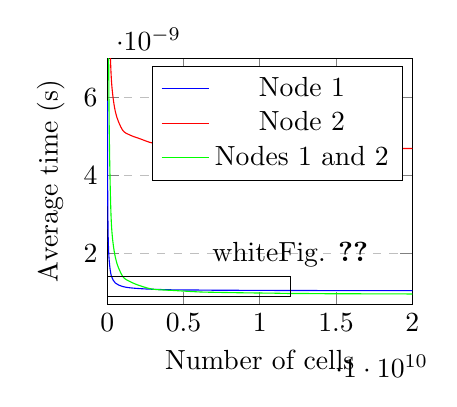
\begin{tikzpicture}
\begin{axis}[
    %title={Average time per cell},
    xlabel={Number of cells},
    ylabel={Average time (s)},
    xmin=0, xmax=20000000000,
    ymin=7e-10, ymax=7e-09,
    legend pos=north east,
    ymajorgrids=true,
    grid style=dashed,
    scaled x ticks={real:10000000000},
    width=0.45\linewidth,
]


\addplot[
    color=blue,
    smooth,
    ]
    coordinates {
    (16777216, 5.9137855257306775e-09)(33554432, 3.600158861705235e-09)(67108864, 2.3944228887557983e-09)(134217728, 1.8066061394555226e-09)(268435456, 1.4282848153795516e-09)(536870912, 1.2414301080363135e-09)(1000000000, 1.152977142857143e-09)(1500000000, 1.119065714285714e-09)(2147483648, 1.0979907321078438e-09)(3000000000, 1.0814785714285714e-09)(4294967296, 1.0668948691870486e-09)(6000000000, 1.0614280952380955e-09)(7000000000, 1.057224693877551e-09)(8589934592, 1.0550598381087185e-09)(10000000000, 1.0521971428571429e-09)(11000000000, 1.0512831168831168e-09)(12000000000, 1.0494261904761902e-09)(13000000000, 1.0495164835164835e-09)(14000000000, 1.0483724489795918e-09)(17179869184, 1.0460199389074528e-09)(25769803776, 1.0433235383104711e-09)(34359738368, 1.042618532665074e-09)(42949672960, 1.0408397897013597e-09)(51539607552, 1.0398679435075748e-09)(60129542144, 1.0400224115927607e-09)(68719476736, 1.0391142235935798e-09)(77309411328, 1.0390710529117357e-09)(85899345920, 1.0391409575406993e-09)(94489280512, 1.0389721250863041e-09)(100000000000, 1.0383371428571429e-09)(103079215104, 1.0382666784737793e-09)(111669149696, 1.038346634051957e-09)(120259084288, 1.0378354666184407e-09)
    };

\addplot[
    color=red,
    smooth,
    ]
    coordinates {
    (16777216, 3.245565720966884e-08)(33554432, 1.8672138452529907e-08)(67108864, 1.1961538876805988e-08)(134217728, 8.379966020584107e-09)(268435456, 6.4965124641145975e-09)(536870912, 5.626971168177468e-09)(1000000000, 5.162437142857143e-09)(1500000000, 5.029282857142857e-09)(2147483648, 4.935963079333305e-09)(3000000000, 4.824004761904761e-09)(4294967296, 4.785867141825813e-09)(6000000000, 4.748461904761905e-09)(7000000000, 4.729608163265305e-09)(8589934592, 4.728251535977636e-09)(10000000000, 4.7160128571428574e-09)(11000000000, 4.704388311688311e-09)(12000000000, 4.696046428571429e-09)(13000000000, 4.699453846153845e-09)(14000000000, 4.695503061224491e-09)(17179869184, 4.688792562644397e-09)(25769803776, 4.678011117946534e-09)(34359738368, 4.6729318065834904e-09)(42949672960, 4.667090252041816e-09)(51539607552, 4.665895609096402e-09)(60129542144, 4.661319378231253e-09)(68719476736, 4.661219593669687e-09)(77309411328, 4.661910694151644e-09)(85899345920, 4.659480016146388e-09)(94489280512, 4.6594083526885355e-09)(100000000000, 4.6598900000000005e-09)(103079215104, 4.659376351074094e-09)(111669149696, 4.6597087530644385e-09)(120259084288, 4.659140748637063e-09)
    };

\addplot[
    color=green,
    smooth,
    ]
    coordinates {
    (16777216, 2.9583752155303957e-08)(33554432, 1.514038017817906e-08)(67108864, 9.290228996958051e-09)(134217728, 5.197258932249886e-09)(268435456, 2.8187840112618036e-09)(536870912, 1.8953390951667517e-09)(1000000000, 1.4202885714285714e-09)(1500000000, 1.277607619047619e-09)(2147483648, 1.1723881055201802e-09)(3000000000, 1.083004761904762e-09)(4294967296, 1.0516730669353688e-09)(6000000000, 1.0138707142857144e-09)(7000000000, 1.003642244897959e-09)(8589934592, 9.929328225553036e-10)(10000000000, 9.85383e-10)(11000000000, 9.808103896103896e-10)(12000000000, 9.733238095238094e-10)(13000000000, 9.729956043956044e-10)(14000000000, 9.68534693877551e-10)(17179869184, 9.647562235061612e-10)(25769803776, 9.547974470825421e-10)(34359738368, 9.519322442689111e-10)(42949672960, 9.487150236964226e-10)(51539607552, 9.463479121526082e-10)(60129542144, 9.423898704045889e-10)(68719476736, 9.409590607642063e-10)(77309411328, 9.429238234010953e-10)(85899345920, 9.43106466106006e-10)(94489280512, 9.422190487384794e-10)(100000000000, 9.425682857142859e-10)(103079215104, 9.416450103301378e-10)(111669149696, 9.416758625225706e-10)(120259084288, 9.41362802167328e-10)
    };

\addplot[
    color=black,
    mark=none,
] coordinates {(0,9e-10) (0,1.4e-09) (12000000000,1.4e-09) (12000000000,9e-10) (0,9e-10)};

\pgfplotsset{
    after end axis/.code={
        \node[above] at (axis cs:12000000000,1.4e-09){\contour{white}{Fig. \ref{result_graph_cell_zoom}}};
    }
}


\legend{Node 1, Node 2, Nodes 1 and 2}
\end{axis}
\end{tikzpicture}
}%
    \subfloat[][Zoomed in]{\label{result_graph_cell_zoom}
\begin{tikzpicture}
\begin{axis}[
    %title={Average time per cell},
    xlabel={Number of cells},
    ylabel={Average time (s)},
    xmin=0, xmax=15000000000,
    ymin=9e-10, ymax=1.4e-09,
    legend pos=north east,
    ymajorgrids=true,
    grid style=dashed,
    scaled x ticks={real:10000000000},
]


\addplot[
    color=blue,
    smooth,mark=diamond,
    ]
    coordinates {
    (16777216, 5.886852741241455e-09)(33554432, 3.59540581703186e-09)(67108864, 2.401748299598694e-09)(134217728, 1.8008887767791747e-09)(268435456, 1.4292880892753601e-09)(536870912, 1.2423399835824965e-09)(1000000000, 1.154624e-09)(2147483648, 1.0980861261487008e-09)(4294967296, 1.067038159817457e-09)(8589934592, 1.0550598381087185e-09)(10000000000, 1.052398e-09)(17179869184, 1.0460199389074528e-09)(25769803776, 1.0433235383104711e-09)(34359738368, 1.042618532665074e-09)(42949672960, 1.0408397897013597e-09)(51539607552, 1.0398679435075748e-09)(60129542144, 1.0400224115927607e-09)(68719476736, 1.0391142235935798e-09)(77309411328, 1.0390710529117357e-09)(85899345920, 1.0391409575406993e-09)(94489280512, 1.0389721250863041e-09)(100000000000, 1.03832e-09)(103079215104, 1.0382666784737793e-09)(111669149696, 1.038346634051957e-09)(120259084288, 1.0377527879817145e-09)
    };

\addplot[
    color=green,
    smooth,mark=square,
    ]
    coordinates {
    (16777216, 2.9002046585083008e-08)(33554432, 1.5357071161270142e-08)(67108864, 9.34590995311737e-09)(134217728, 5.2753239870071416e-09)(268435456, 2.741926163434982e-09)(536870912, 1.903323084115982e-09)(1000000000, 1.4446680000000001e-09)(2147483648, 1.1591557413339615e-09)(4294967296, 1.056760549545288e-09)(8589934592, 9.929328225553036e-10)(10000000000, 9.83829e-10)(17179869184, 9.647562235061612e-10)(25769803776, 9.547974470825421e-10)(34359738368, 9.519322442689111e-10)(42949672960, 9.487150236964226e-10)(51539607552, 9.463479121526082e-10)(60129542144, 9.423898704045889e-10)(68719476736, 9.409590607642063e-10)(77309411328, 9.429238234010953e-10)(85899345920, 9.43106466106006e-10)(94489280512, 9.422190487384794e-10)(100000000000, 9.424657999999999e-10)(103079215104, 9.416450103301378e-10)(111669149696, 9.416758625225706e-10)(120259084288, 9.416818751820496e-10)
    };

\addplot[
    color=indigo,
    smooth,
    ]
    coordinates {
    <generator object <genexpr> at 0x7f11cfe1e410>
    };


\legend{Node 1, Nodes 1 and 2}
\end{axis}
\end{tikzpicture}
}
    \caption{Average time per cell} \label{result_graph_cell_total}
\end{figure*}

\section{Testing the performance} \label{testing}
The implementation has been tested on a cluster of two nodes.
%The test will compare the performance of each single node to the performance of the nodes working together.
%Therefore the exact specifications of the nodes will not be discussed, as the nodes will not be compared nodes to each other.%
Node 1 has an Nvidia GPU with a maximum work-group size of 1024 and Node 2 has an AMD GPU with a maximum work-group size of 256.
That means that the $width$, as discussed in \cref{algorithms}, are 1024 and 256 on Nodes 1 and 2 respectively.
The implementation has been run on the nodes separately and on the nodes as a cluster.
This allows us to compare the time the program needs to return the result.
The values used in figures \ref{result_graph_total} and \ref{result_graph_cell_total} are averages of ten separate runs.
The x-axes represents the product of the lengths of the sequences compared, which is equal to the number of cells in the solution matrix as mentioned in \cref{originalalg}.
The y-axes represents the average time it takes to solve the problem in \cref{result_graph_total} and the average time it takes for one cell to be computed in \cref{result_graph_cell_total}.

\Cref{result_graph_total} shows that the implementation works faster on a cluster than on the individual nodes if the number of cells becomes larger than approximately $0.4 \cdot 10^{10}$ cells.
It also shows that Node 2 takes longer than Node 1 to solve the problem.
This is due to the fact that the width of Node 2 is smaller than the width of Node 1.
If the number of cells is equal to $1.0 \cdot 10^{10}$ Node 1 takes 10.5 seconds to complete, Node 2 takes 47.2 seconds to complete and the cluster takes 9.8 seconds to complete.
The width used in Node 1 is four times as big as the width in Node 2, but the time required to solve the problem is 4.50 times as long.
Therefore we can conclude that Node 2 will be the bottleneck in the cluster.
The implementation does not take into account the difference in performance between nodes, so Node 2 defines the maximum performance of the cluster.

The total width of the cluster is equal to $1024 + 256 = 1280$, and the width of Node 2 is 256.
So Node 2 is going to handle $256 / 1280 = \frac{1}{5}$ of the pillars.
That means that the time the cluster should take is at least one fifth of the time it takes Node 2 to solve the problem.
There is however a small difference between $47.2 / 5.0 = 9.44$ and $9.8$.
This is probably due to the fact that the use of a cluster takes more time to setup and the communication provides some overhead.

The setup taking more time can be seen in \cref{result_graph_cell_total}.
These graphs show the time taken per cell, so extra time taken independent of the number of cells will be visible in these graphs.
The steep decline in time per cell at the left side of the graph is a clear indication that the time to setup is indeed significant.
In these graphs it is also visible that the cluster becomes faster than Node 1 at approximately $0.4 \cdot 10^{10}$ cells, as the amount of time per cell in the cluster drops below the time per cell in Node 1.

From these results we can conclude that optimal number of GPUs in a cluster depend on the size of the sequences compared, when considering the speed of the calculation.
For the specific cluster used in this section $0.4 \cdot 10^{10}$ cells is the size when the cluster is faster than the individual nodes.
The cluster will however never be more efficient than the individual nodes, as the overhead on a cluster persist no matter the size of the cluster.
This means that the user should consider whether or not the superior speed outweighs the inferior efficiency.
\todo{max performance}

\subsection{Comparison of algorithms}
Comparison with the algorithm of De Heus is not useful, since it can not solve the edit distance of sequences longer than the $width$ of a node \cite{Heus}.
The implementation of this paper does not focus on such small sequences, as extra complexity and features results in a significant overhead while computing them.
It is save to say that for comparing small sequences the algorithm of De Heus is more suitable.


\begin{comment}
\subsection{Comparison with CPU implementations}
Comparing the implementation with CPU based algorithms is also not useful, as there is no reliable method to compare the performance of CPUs with GPUs apart from running the implementation on each of them.
The difference between CPUs and GPUs is significantly

A more expensive device will not necessarily have a better performance, so even the cost does not serve as a reliable benchmark.

Even the cost of the devices is not a reliable benchmark as manufacturers do not publish the production cost of a device and use different profit margins.
That is why no such comparison is included.
\end{comment}
